\documentclass[9pt,twocolumn]{article}





\usepackage{graphicx}
\usepackage{natbib}
\bibliographystyle{unsrtnat}
\usepackage{lmodern}
\usepackage{amssymb,amsmath}
\usepackage{ifxetex,ifluatex}
\usepackage{fixltx2e} % provides \textsubscript
\ifnum 0\ifxetex 1\fi\ifluatex 1\fi=0 % if pdftex
  \usepackage[T1]{fontenc}
  \usepackage[utf8]{inputenc}
\else % if luatex or xelatex
  \ifxetex
    \usepackage{mathspec}
    \usepackage{xltxtra,xunicode}
  \else
    \usepackage{fontspec}
  \fi
  \defaultfontfeatures{Mapping=tex-text,Scale=MatchLowercase}
  \newcommand{\euro}{€}
  \fi
  \usepackage{wrapfig}
% use upquote if available, for straight quotes in verbatim environments
\IfFileExists{upquote.sty}{\usepackage{upquote}}{}
% use microtype if available
\IfFileExists{microtype.sty}{%
\usepackage{microtype}
\UseMicrotypeSet[protrusion]{basicmath} % disable protrusion for tt fonts
}{}
\ifxetex
  \usepackage[setpagesize=false, % page size defined by xetex
              unicode=false, % unicode breaks when used with xetex
              xetex]{hyperref}
\else
  \usepackage[unicode=true]{hyperref}
  \fi

%  \usepackage[T1]{fontenc}
\renewcommand{\rmdefault}{ptm}
\usepackage{fourier}

\usepackage[scaled=0.875]{helvet} % ss
\renewcommand{\ttdefault}{pcr} %tt

\usepackage[dvipsnames]{xcolor}
\hypersetup{breaklinks=true,
            bookmarks=true,
            pdfauthor={},
            pdftitle={},
            colorlinks=true,
            citecolor=blue,
            urlcolor=blue,
            linkcolor=magenta,
            pdfborder={0 0 0}}
\urlstyle{same}  % don't use monospace font for urls
\setlength{\parindent}{0pt}
\setlength{\parskip}{6pt plus 2pt minus 1pt}
\setlength{\emergencystretch}{3em}  % prevent overfull lines

\usepackage{lastpage}
\usepackage{fancyhdr}
\pagestyle{fancy}

\rhead{} \chead{}\lhead{}
\cfoot{}

\fancyfoot[LE,RO]{page~\thepage~of~\pageref{LastPage}}
\fancyfoot[LO,RE]{\rotatebox[origin=c]{180}{\copyright} 2015, Tim Menzies, sort of.}



  \renewcommand{\footrulewidth}{0.4pt}

\date{}
%\usepackage{times}
\usepackage[margin=0.65in,landscape]{geometry}

\makeatletter
\newcommand{\verbatimfont}[1]{\def\verbatim@font{#1}}%
\makeatother
\usepackage{fancyvrb}


\usepackage[shortlabels]{enumitem}
\setlist{nosep}

\DefineVerbatimEnvironment%
  {MyVerbatim}{Verbatim}
  {numbers=right,numbersep=2mm,firstnumber=last,stepnumber=1,xleftmargin=12pt,xrightmargin=24pt,
   frame=lines,framerule=0.1mm,fontsize=\scriptsize,rulecolor=\color{Gray}}

  \definecolor{britishracinggreen}{rgb}{0.0, 0.26, 0.15}
  \definecolor{bulgarianrose}{rgb}{0.28, 0.02, 0.03}
  \definecolor{coolblack}{rgb}{0.0, 0.18, 0.39}
  \definecolor{mygreen}{rgb}{0,0.6,0}
  \definecolor{mymauve}{rgb}{0.58,0,0.82}
  
  \usepackage{listings}

  \colorlet{shadecolor}{gray!8}
  \lstset{% general command to set parameter(s)
    language=Python,
    firstnumber=last,
    xleftmargin=6pt,
    xrightmargin=12pt,
    numberblanklines=false,
    backgroundcolor = \color{shadecolor},
    numbers=right, stepnumber=1, numberstyle=\tiny, numbersep=1pt,
    basicstyle=\linespread{0.90}\scriptsize\ttfamily, % print whole listing small
    keywordstyle=\color{coolblack}\bfseries,
    emphstyle=\ttb\color{bulgarianrose},    % Custom highlighting style
    stringstyle=\color{britishracinggreen},
    commentstyle=\color{red},
    stringstyle=\color{mygreen},
    %frame=tb,framerule=0.5pt,rulecolor=\color{Gray},
      showstringspaces=false,
    } % no special string spaces

 \newcommand{\said}[1]{\citet*{#1}}


 \hypersetup{linkcolor=black}
\setcounter{tocdepth}{2}

\newcommand{\eq}[1]{Equation~\ref{eq:#1}}
\newcommand{\bi}{\begin{itemize}}
\newcommand{\ei}{\end{itemize}}
\newcommand{\be}{\begin{enumerate}}
\newcommand{\ee}{\end{enumerate}}
\newcommand{\tion}[1]{\textsection\ref{sec:#1}}
\newcommand{\fig}[1]{Figure~\ref{fig:#1}}

\setlength{\columnsep}{10mm}
\setlength{\columnseprule}{0.1pt}

\renewcommand{\headwidth}{10in}
%% \makeatletter
%%     \def\headrule{{\if@fancyplain\let\headrulewidth\plainheadrulewidth\fi
%%         \hrule\@height\headrulewidth\@width 7in \vskip-\headrulewidth}}
%% \makeatother

%% \makeatletter
%%     \def\footrule{{\if@fancyplain\let\headrulewidth\plainheadrulewidth\fi
%%         \hrule\@height\headrulewidth\@width 7in \vskip-\headrulewidth}}
%% \makeatother

\usepackage{tocloft}

\setlength{\cftbeforesecskip}{6pt}

\usepackage{moresize}



\newcommand{\parting}[2]{\newpage
\onecolumn
\clearpage
\fancyhead[LE,RO]{}
\fancyhead[LO,RE]{}
\vspace*{\fill}
\begin{center}
  \addcontentsline{toc}{section}{#1~~~#2}
  \begin{minipage}{.6\textwidth}
    \begin{center}
      { \fontsize{450}{450} \selectfont {\bf #1}}\\~\\ \LARGE{(#2)}\end{center}
\end{minipage}
\end{center}
\vfill % equivalent to \vspace{\fill}
\clearpage
\fancyhead[LE,RO]{\slshape \rightmark}
\fancyhead[LO,RE]{\slshape \leftmark}
\twocolumn
}
  
  
\begin{document} 

%\renewcommand{\verbatim@font}{\ttfamily\small}

\onecolumn
\title{
  {\bf \HUGE{Evil Code for Wicked Problems, part 4}}\\~\\~\\
    \fcolorbox{red}{white}{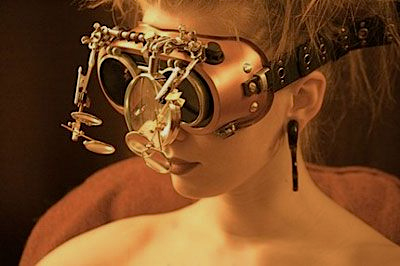
\includegraphics[width=6.5in]{img/herGoggles.png}}\\
    \Large{A Research Programmer's Guide to World Domination-- in Python.}\\
    \Large{a.k.a. {\em Lecture Notes, Automated
  SE}, CS, NC State, Fall'15}}
\author{by Tim Menzies \\\#attentionDeficitSquirrel\\Download:
  see {\tt book.pdf} at https://github.com/txt/evil\\This version: \today}
   

\maketitle
\thispagestyle{empty}

\clearpage
\small
\twocolumn

\pagestyle{fancy}



 \subsection*{About this book} This book is a  ``how to'' guide about model-based reasoning using
   data mining and search-based tools (with examples taken from software engineering).
   It is intended for graduate  students taking
  a one semester subject in advanced programming methods as
  well as researchers developing the next generation
  of model-based reasoning tools.  

  Using Python 2.7, the book builds (from the ground up) numerous
  tiny tools that can tame seemingly complex
  tasks. The combined toolkit, called RINSE, offers four kinds of functionality:
  \be
  \item
    It {\em \underline{r}epresents}  models using domain-specific languages;
    \item It supports
    {\em \underline{in}ference} across the multiple goals of those models using multi-objective optimization.
    \item It shows how to succinctly {\em \underline{s}ummarize} that inference  using data miners;
    \item It has  many tools for the
   {\em \underline{e}valuation} of different inference methods. 
   \ee
   
   RINSE is a not some shiny  end-user click-and-point GUI package.
   Rather, it is a starter-kit that demonstrates an novel  model-based approach to problem solving where programmers
   mix and match and extend data miners and multi-objective optimizers.

   RINSE was written using the mantra ``less is more''. Whenever it was found that small parts of the
   the code handled most 
   of the functionality, then the extra functionality was ejected. This resulted in a (very) small code base
   which can be readily browsed, learned, taught, and changed.


   \vfill


   \subsection*{Content Advisory }
\begin{wrapfigure}{r}{1.5in}
  
\includegraphics[width=1.5in]{img/shark.jpg}
  \end{wrapfigure}
This book contains strong language, weakly typed (and tapped with glee).

This book may contain excessive or gratutious fun--
as well as ideas that some readers may (or may not) find disturbing.
This book does not necessarily 
believed or endorse those ideas- but plays with them anyway
(and asks you to do the same).

This book may include heresies, not suitable for anyone  who believes in established wisdom, without
adequate experimentation. It is
intended for mature audiences only; i.e.  those
old enough to know there is much left to know. 

This book may (or may not) contain peanuts or tree nut products.

Batteries not included.

\newpage

\tableofcontents

\newpage

   
\subsection*{Source Code Availability and Copyleft}
To download the RINSE code, see http://github.com/txt/mase.
The software associated with this book
is free and unencumbered and released into the public domain. 

Anyone is free to copy, modify, publish, use, compile, sell, or
distribute this software, either in source code form or as a compiled
binary, for any purpose, commercial or non-commercial, and by any
means.

In jurisdictions that recognize copyright laws, the author or authors
of this software dedicate any and all copyright interest in the
software to the public domain. We make this dedication for the benefit
of the public at large and to the detriment of our heirs and
successors. We intend this dedication to be an overt act of
relinquishment in perpetuity of all present and future rights to this
software under copyright law.

THE SOFTWARE IS PROVIDED "AS IS", WITHOUT WARRANTY OF ANY KIND,
EXPRESS OR IMPLIED, INCLUDING BUT NOT LIMITED TO THE WARRANTIES OF
MERCHANTABILITY, FITNESS FOR A PARTICULAR PURPOSE AND NONINFRINGEMENT.
IN NO EVENT SHALL THE AUTHORS BE LIABLE FOR ANY CLAIM, DAMAGES OR
OTHER LIABILITY, WHETHER IN AN ACTION OF CONTRACT, TORT OR OTHERWISE,
ARISING FROM, OUT OF OR IN CONNECTION WITH THE SOFTWARE OR THE USE OR
OTHER DEALINGS IN THE SOFTWARE.

For more information, please refer to http://unlicense.org

\vfill

   \subsection*{About the Author}

\begin{wrapfigure}{r}{1.5in}
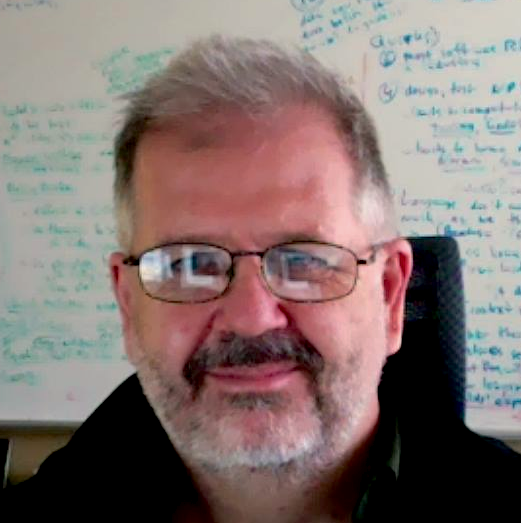
\includegraphics[width=1.5in]{img/tim.png}
\end{wrapfigure}
Tim Menzies (Ph.D., UNSW, 1995, http://menzies.us) is a full Professor in CS at North Carolina State University where he teaches software engineering and automated software engineering. His research relates to synergies between human and artificial intelligence, with particular application to data mining for software engineering.

In his career, he has been a lead researcher on projects for NSF, NIJ, DoD, NASA, USDA, as well as joint research work with private companies.
He is the author of over 230 referred publications; and is one of the 100 most cited authors in software engineering out of over 80,000 researchers.

Prof. Menzies is an associate editor of IEEE
Transactions on Software Engineering, Empirical
Software Engineering and the Automated Software
Engineering Journal. His community service includes
co-founder of the PROMISE project (storing data for repeatable SE
experiments);
co-program chair for the 2012 conference on Automated SE and the 2015
New Ideas and Emerging Research track at the International Conference on SE;
and 
co-general chair for 2016 International Conference on Software Maintenance and Evolution.

Prof. Menzies can be contacted at \verb!tim.menzies@gmail.com!.




\newpage




%\renewcommand\contentsname{}



\parting{A}{An Introduction}
\section{Welcome to the Evil Plan}\label{welcome-to-the-evil-plan}

\textbf{``The world is a dangerous place to live, not because of the
people who are evil, but because of the people who don't do anything
about it.''} - Albert Einstein

The evil plan (by programmers) to take over the world is progressing
nicely. Certain parts of that plan were initially somewhat undefined.
However, given recent results, this book can now fill in the missing
details from part4 of that plan.

But first, a little history. As all programmers know, the initial parts
of the plan were completed years ago. Part one was was programmers to
adopt a meek and mild persona (possibly even boring and dull).

Part two was, under the guise of that persona, ingratiated ourselves to
government and indistrial agenices (education, mining, manufacturing,
etc etc). Once there, make our work essential to their day to day
opertion. Software is now a prime driven in innovation and all aspects
of economic development. Software mediates most aspects of our daily
lives such as the stock market models that control the economy; the
probablistic models that recommend what books to read; and the
pacemakers that govern the beating of our heart.

After that, part three was to make more material available for our
inspection and manipluation. To this end, the planet was enclosed a
digital network that grants us unprecendented access to petabytes of
sensors and effectors. Also, by carefully seeding a few promienet
examples of successful programmers (Gates, Jobs, Zuckerburg, thanks
guys!), we convinced a lot of people to write lots of little tools, each
of which represent or control some thing, somewhere.

Part four was a little tricky but, as shown in this book, it turned out
not to be too hard. Having access to many models and much data can be
overwhelming-- unless some GREAT SECRET can be used to significantly
simply all that information. For the longest time, that GREAT SECRET was
unknown. However, recent advances have revealed that if we describe
something in \emph{N} dimensions, then there is usually a much smaller
set of \emph{M} dimensions that contain most of the signal. So GREAT
SECRET is that is it very easy (and very fast) to find then exploit
those few number of \emph{M} dimensions for solving seemingly complex
problems.

\begin{wrapfigure}{r}{1.3in}

\includegraphics[width=1.3in]{img/evillaugh.jpg}
\end{wrapfigure}

With those controllers in hand, we are now free to move to part five;
i.e.~taking over the world. The truly evil part of this work is this:
\emph{now you know you have the power to change the world}. This also
means that (evil laugh) \emph{now you have the guilt if you do not use
that power to right the wrongs of the world}. So welcome to a lifetime
of discontent (punctuated by the occasionaly, perhaps fleerting,
truimphs) as you struggle to solve a very large number of pressing
problems facing humanity.

'Nough said. Good luck with that whole world domination thing. One tip:
if at first you cannot dominate the whole thing, start out with
something smaller. Find some people who have problems, then work with
them to make changes that help them. Remember: if you don't try then you
won't be able to sleep at night. Ever again (evil laugh).

\newpage
\subsection{Research Programming}\label{research-programming}

Silliness aside, this book is about how to be a \emph{research
programmer}. Research programmer's understand the world by:

\begin{itemize}
\itemsep1pt\parskip0pt\parsep0pt
\item
  Codify out current understanding of ``it'' into a model.
\item
  Reasoning about the model.
\end{itemize}

We take this term ``research programmer'' from Ph.D.~Steve Guao's 2012
dissertation.

\subsubsection{Challenges with Research
Programming}\label{challenges-with-research-programming}

Research programming sounds simple, right? Well, there's a catch
(actually, there are several catches).

Firstly, models have to be written and it can be quite a task to create
and validate a model of some complex phenomenon.

see also list in sbse14

Secondly, many models related to \emph{wicked problems};
i.e.\textasciitilde{}problems for which there is no clear best solution.
Tittel XXXWorse still, some models relate to \_wicked there is final
matter of the \emph{goals} that humans want to achieve with those
models. When those goals are contradictory (which happens, all too
often), then our model-based tools must negotiate complex trade offs
between different possibilities.

Thirdly, if wicked problems were not eough, there is also the issue of
uncertainty. Many real world models contain large areas of uncertainty,
especially if that model relates to something that humans have only been
studying for a few decades.

Fourthly, even if you are still not worried about the effectiveness of
reserach problem, consider the complexity of real-world phenomonem. Many
of these models are so complex that we cannot predict what happens when
the parts of that model interact.

Sounds simple, right? Well, there's a catch. Many models related to
\emph{wicked problems}; i.e.~problems for which there is no clear best
solution. Tittel XXXWorse still, some models relate to \_wicked there is
final matter of the \emph{goals} that humans want to achieve with those
models. When those goals are contradictory (which happens, all too
often), then our model-based tools must negotiate complex trade offs
between different possibilities.

If wicked problems were not eough, there is also the issue of
uncertainty. Many real world models contain large areas of uncertainty,
especially if that model relates to something that humans have only been
studying for a few decades.

And if you are still not worried about the effectiveness of reserach
problem, consider the complexity of real-world phenomonem. Many of these
models are so complex that we cannot predict what happens when the parts
of that model interact.

\subsubsection{Parts}\label{parts}

\begin{itemize}
\itemsep1pt\parskip0pt\parsep0pt
\item
  Domain specifc langauges (representation)
\item
  execution (nuktu-objective ootiization)
\item
  evaluation (statistical methods for experimental sciencetists in SE)
\item
  Philophsopy (about what it means to know, and to doubt)
\end{itemize}

\subsubsection{Implications for Software
Engineering}\label{implications-for-software-engineering}

Note that research programming changes the nature and focus and role of
21st century software engineering:

\begin{itemize}
\itemsep1pt\parskip0pt\parsep0pt
\item
  Traditionally, software engineering is about services that meet
  requirements.
\item
  But with research programming, software engineering is less about
  service than about search. Research programming's goal is the
  discovery of interesting features in existing models (or perhaps even
  the evolution of entirely new kinds of models).
\end{itemize}

For example, old-fashioned software engineerings might explore small
things like strings or ``hello world''. But with research programmers
explore \textbf{BIG} things like String Theory or ``hello world model of
climate change and economic impacts''.



\subsection*{The GREAT SECRET}

\subsection*{Example}

brook's law.  DSL in python of CM. data mining.

\parting{B}{Before we begin}

\section{Before we Begin}\label{before-we-begin}

Our goals are lofty- introducing a new paradigm that combines data
mining with multi-objective optimization. And doing so in such a way
that even novices can understand, use, and adapt these tools for a large
range of new tasks.

But before we can start all that, we have to handle some preliminaries.
All artists, and programmers, should start out as apprentices. If we
were painters and this was Renaissance Italy, us apprentices would spend
decades study the ways of the masters, all the while preparing the
wooden panels for painting; agrinding and mixing pigments; drawing
preliminary sketches, copying paintings, and casting sculptures. It was
a good system that gave us the Michelangelo and Da Vinci who, in turn,
gave us the roof of the Sistine Chapel and the Mona Lisa.

In terms of this book, us apprentices first have to become effective
Python programmers. The rest of this chapter offers:

\begin{itemize}
\itemsep1pt\parskip0pt\parsep0pt
\item
  Some notes on useful web-based programming tools
\item
  Some pointers on learning Python
\item
  Some start-up exercises to test if you have an effective Python
  programming environment.
\end{itemize}

\subsection{Useful On-Line Tools}\label{useful-on-line-tools}

This book was written using the following on-line tools. There exists
many other great, readily available, tools. So if you know of better
ones, then please let me know (then maybe I'll switched to your tool
stack).

\subsubsection{Stackoverflow}\label{stackoverflow}

To find answers to nearly any question you'll ever want to ask about
Python, go browse:

\begin{lstlisting}
 http://stackoverflow.com/questions/tagged/python
\end{lstlisting}

\subsubsection{Github}\label{github}

All programmers should use off-site backup for their work. All
programmers working in teams should store their code in repositories
that let them fork a branch, work separately, then check back their
changes into the main trunk.

There are many freely-available repository tools. Github is one such
service that supports the \texttt{git} repository tool. Github has some
special advantages:

\begin{itemize}
\itemsep1pt\parskip0pt\parsep0pt
\item
  It is the center of vast social network of programmers;
\item
  Github support serving static web sites straight from your Github
  repo.
\item
  Many other services offer close integration with Github (e.g.~the
  Cloud9 tool discussed below).
\end{itemize}

For more information, go to:

\begin{lstlisting}
 http://github.com
\end{lstlisting}

The good news about Github is that it is very easy to setup and
configure. The bad news is that each Github repository has a 1GB size
limit. But that is certainly enough to get us started.

For Linux/Unix/Mac users, I add the following tip. In each of your
repository directories, add a \texttt{Makefile} with the following
contents.

\begin{lstlisting}
typo:   ready
        @- git status
        @- git commit -am "saving"
        @- git push origin master # update as needed

commit: ready
        @- git status
        @- git commit -a
        @- git push origin master

update: ready
        @- git pull origin master

status: ready
        @- git status

ready:
        @git config --global credential.helper cache
        @git config credential.helper \
             'cache --timeout=3600'

timm:  # <== change to your name
        @git config --global user.name "Tim Menzies"
        @git config --global user.email \
                      tim.menzies@gmail.com
\end{lstlisting}

This \texttt{Makefile} implements some handy shortcuts:

\begin{itemize}
\itemsep1pt\parskip0pt\parsep0pt
\item
  \texttt{make\ typo} is a quick safety save-- do this many times per
  day;
\item
  \texttt{make\ commit} is for making commented commits-- use this to
  comment any improvements and/or degradation of functionality.
\item
  \texttt{make\ update} is for grabbing the latest version off the
  server-- do this at least at the start of each day.
\item
  \texttt{make\ status} is for finding files that are not currently
  known to Github.
\item
  \texttt{make\ ready} remembers your Github password for one hour-- use
  this if you use \texttt{make\ typo} a lot and you want to save some
  keystrokes.
\item
  \texttt{make\ timm} should be used if Github complains that it does
  not know who you are. Before running this one, edit this rule to
  include your name and email.
\end{itemize}

Tip:

\begin{itemize}
\itemsep1pt\parskip0pt\parsep0pt
\item
  IMPORTANT: When writing a \texttt{Makefile}, all indentations have to
  be made using the tab character, not 8 spaces.
\end{itemize}

Of course, there are 1000 other things you can do with a
\texttt{Makefile}. For example, this book is auto-generated by a
\texttt{Makefile} that automatically extracts comments and code from my
Python source code, then compiles the comments as Markdown, then used
the wonderful \texttt{pandoc} tool to compile the Markdown into Latex,
then converts the Latex to a \texttt{.pdf} file. Which is all
interesting stuff-- but beyond the scope of this book.

\subsubsection{Cloud9}\label{cloud9}

If you do not want to install code locally on your machine, then there
are many readily-available on-line integrated development environments.

For example, to have root access to a fully-configured Unix
installation, you could go to

\begin{lstlisting}
 http://c9.io
\end{lstlisting}

One tip is to host your Cloud9 workspace on Github. As of June 2015, the
procedure for doing that was:

\begin{itemize}
\itemsep1pt\parskip0pt\parsep0pt
\item
  Go to Github and create an empty repository.
\item
  Log in to Cloud9 using your GitHub username (at \texttt{http://c9.io},
  there is a button for that, top right).
\item
  Hit the green \emph{CREATE NEW WORKSPACE} button

  \begin{itemize}
  \itemsep1pt\parskip0pt\parsep0pt
  \item
    Select \emph{Clone from URL};
  \item
    Find \emph{Source URL} and enter in
    \texttt{http://github.com/you/yourRepo}
  \item
    Wait ten seconds for the screen to change.
  \item
    Hit the green \emph{START EDITING} button.
  \end{itemize}
\end{itemize}

This will drop you into the wonderful Cloud9 integrated development
environment. Here, you can edit code and (using the above
\texttt{Makefile}) run \texttt{make\ typo} to backed up your code
outside Cloud9, over at \texttt{Github.com} (which means that if ever
Cloud9 goes away, you will still have your code).

The good news about Cloud9 is that it is very easy to setup and
configure. The bad news is that each Cloud9 workspace has the same
limits as Github- a 1GB size limit. Also, for CPU-intensive
applications, shared on-line resources like Cloud9 can be a little slow.
That said, for the newbie, Cloud9 is a very useful tool to jump start
the learning process.

\subsection{Learning Python}\label{learning-python}

\subsubsection{Why Python?}\label{why-python}

I use Python for two reasons: readability and support. Like any computer
scientist, I yearn to use more powerful languages like LISP or
Javascript or Haskell (Have you tried them? They are \emph{great}
languages!). That said, it has to be said that good looking Python
\emph{reads} pretty good-- no ugly brackets, indentation standards
enforced by the compiler, simple keywords, etc.

Ah, you might reply, but what about other beautiful languages like
CoffeeScipt or Scala or insert yourFavoriteLanguageHere? It turns out
that, at the time of this writing, that there is more tutorial support
for Python that any other language I know. Apart from the many excellent
Python textbooks, the on-line community for Python is very active and
very helpful; e.g.~see stackoverlow.com.

\subsubsection{Which Python?}\label{which-python}

This book uses Python 2.7, rather than the latest-and-greatest version,
which is called Python3. Why?

The problems with Python3 are well-documented and being actively
addressed by the Python community. In short, many large and useful
Python libraries are not yet unavailable in Python3 so many developers
are sticking with the older version.

This situation may change in the near future so, in the coding standards
discussed below, we discuss how to use Python3 idioms while coding in
Python2. This will make our eventual jump to Python3 much easier.

\subsubsection{Installing}\label{installing}

To get going on Python, you will need a \emph{good} Python environment.
You may already have a favorite platform or interactive development
environment, in which case you can use that (and if not, you might
consider using the Cloud9 environment discussed above). To check if your
Python environment is \emph{good}, try changing and installing some
things.

Note that I use Mac/Linux/Unix so all the examples in this book will be
from a Unix-ish command-line prompt. For Windows users, you can

\begin{itemize}
\itemsep1pt\parskip0pt\parsep0pt
\item
  Use Google to find equivalent instructions for your platform;
\item
  Use Cloud9 (simple!).
\item
  Install a Linux in a virtual environment on top of Windows; e.g.~using
  VirtualBox and Ubuntu (warning: not so simple).
\end{itemize}

\paragraph{Code Indentation}\label{code-indentation}

Firstly, change the code indent to 2 spaces. Many editors have this
option.

\begin{itemize}
\itemsep1pt\parskip0pt\parsep0pt
\item
  For the editor I use (EMACS), that magic setting can be found the
  \texttt{add-hock\ \textquotesingle{}python-model-hook} of
  \texttt{.emacs} (available on-line at
  \texttt{https://github.com/timm/timmnix} in the \texttt{dotemacs}
  file).
\item
  For the ACE editor (used in Cloud9), hit the settings button (little
  wheel, top right) \#\#\#\# Get the Package Managers
\end{itemize}

Secondly, make sure you have installed the \texttt{pip} and
\texttt{easy\_install} tools (these are tricks for quickly compiling
Python code). Try running

\begin{lstlisting}
pip -h
easy_install -h
\end{lstlisting}

Tips:

\begin{itemize}
\item
  If these are not installed them Google for installation instructions.
  See also \texttt{https://pypi.python.org/pypi/setuptools} (which has
  hints for Windows users as well as those using Linix/Unix/Mac).
\item
  If you ever run this code and you get permission errors or some notice
  that you cannot update some directories, then run as superuser (by the
  way, one nice thing about Cloud9 is that you have superuser permission
  on your workspaces). To run code as superuser, in Linux/Unix/Mac,
  preface with \texttt{sudo}; e.g. \texttt{sudo\ pip} or
  \texttt{sudo\ pip\_install}

  sudo pip sudo easy\_install
\end{itemize}

\paragraph{Use the Package Managers}\label{use-the-package-managers}

Thirdly, do some installs of various packages. Note that we will make
extensive use of all of the following.

Package1: enable a \emph{watcher} on files that are being edited. Every
time you save the \emph{watched} file, it is re-executed (so you get
rapid feedback on your progress):

\begin{lstlisting}
sudo pip install rerun
\end{lstlisting}

Example: establish a \emph{watch} on \texttt{lib.py}:

\begin{lstlisting}
rerun "python lib.py"
\end{lstlisting}

Package2: 2D plotting with \texttt{matplotlib}

\begin{lstlisting}
sudo pip install matplotlib
\end{lstlisting}

Example: the code, from the \texttt{rinse} repo, shows how to generate a
plot within Cloud9 using \texttt{matplotlib}.

\begin{lstlisting}
# demoMatplot.py                           TRICKS
import matplotlib
matplotlib.use('Agg')     #.................... 1
import matplotlib.pyplot as plt 

def lines(xlabel, ylabel, title,
          f="lines.png",   #................... 2
          xsize=5,ysize=5,lines=[]): 
  width = len(lines[0][1:])
  xs = [x for x in xrange(1,width+1)] 
  plt.figure(figsize=(xsize,ysize))  #......... 3
  plt.xlabel(xlabel)
  plt.ylabel(ylabel) 
  for line in lines: 
    plt.plot(xs,  line[1:],  #................. 4a
                 label = line[0])   #.......... 4b
   
  plt.locator_params(nbins=len(xs)) #.......... 5
  plt.title(title)
  plt.legend()
  plt.tight_layout()                #.......... 6
  plt.savefig(f)

lines("days","production",  #.................. 7
      "Fruit output",
      xsize=3,ysize=3,lines=[
      ["apples",4,3,2,1],
      ["oranges",9,4,1,0.5]])
\end{lstlisting}

If the code works you should see the following file \texttt{lines.out}:

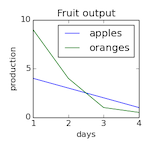
\includegraphics{img/matplotlib101.png}.

The comments in this code show several tricks for such plotting:

\begin{enumerate}
\def\labelenumi{\arabic{enumi}.}
\itemsep1pt\parskip0pt\parsep0pt
\item
  Add this line \emph{right after} importing \texttt{matplotlib}. If
  absent, then when used in a non-X-server environment (e.g.~Cloud9),
  the code crashes.
\item
  Note the use of default parameters. By default, this function writes
  to \texttt{lines.png} but this can be changed when the function is
  called.
\item
  Here we can change the default size of a plot (which defaults to five
  inches square-- do you know why? hint: look at the default parameters
  of the function).
\item
  The line label and the line data is pulled from the data passed to the
  function. To see that, have a look at the last like of the code where
  \texttt{orange} is the first item in the list and the rest is data.
\item
  This is a hack to stop \texttt{matplotlib} adding in ticks like
  ``1.5''. With this hack, the number of ticks is equal to the number of
  items in each line to be plotted.
\item
  Another hack. Once we resize a plot, sometimes the label text gets cut
  off. The fix is to use a \texttt{tight\textbackslash{}\_layout}.
\item
  A sample call to this function.
\end{enumerate}

\subsubsection{Python 101}\label{python-101}

There are many great tools for learning Python, including all the
on-line tools listed above.

In terms of a textbook, I highly recommend \emph{How to Think Like a
Computer Scientist} by Allen Downey, which can be purchased as a paper
book or viewed or downloaded from
\texttt{www.greenteapress.com/thinkpython}. All the source code from
that book is available on-line at:

\begin{lstlisting}
 https://github.com/AllenDowney/ThinkPython
\end{lstlisting}

If you liked that book, it would be good manners to make a small
donation to Prof.~Downey at that website-- but that is entirely up to
you.

Note that there are Python3 versions of this code, available on the web.
Try to avoid those.

In terms of a three week teach yourself program, I recommend the
following.

\begin{itemize}
\itemsep1pt\parskip0pt\parsep0pt
\item
  \textbf{Week1} Read chapters one to four. \emph{Do} exercises
  3.1,3.2,3.3,3.4,3.5. \emph{Do} install \texttt{Swampy} \emph{Do}
  exercise 4.2,4.3 (but makeIn terms of a three-week teach-= yoAt the
  time of this writing, at
\end{itemize}

tutorial mater

\subsubsection{Installing a ``Good'' Python
Environment}\label{installing-a-good-python-environment}

\subsubsection{Python Standards}\label{python-standards}

This textbook uses Python 2.7 for its code base. Of course, it is
tempting to use Python3 but there are still too many Python packages out
there t

\subsection{Mantras}\label{mantras}

\subsubsection{\texorpdfstring{``Do go coding, go for
feedback''}{Do go coding, go for feedback}}\label{do-go-coding-go-for-feedback}

\subsubsection{\texorpdfstring{``Red, Green,
Refactor''}{Red, Green, Refactor}}\label{red-green-refactor}

\subsubsection{\texorpdfstring{``Write Less
Code''}{Write Less Code}}\label{write-less-code}

Holzmann. true

\subsubsection{\texorpdfstring{``Stop writing
classes''}{Stop writing classes}}\label{stop-writing-classes}

Jack Diederich

\subsection{Homework}\label{homework}

\subsubsection{Homework1}\label{homework1}

\begin{itemize}
\itemsep1pt\parskip0pt\parsep0pt
\item
  Do: get an account at \texttt{http://github.com}. Hand-in: your Github
  id.
\item
  Show that you have a \emph{good} Python environment by installing
\end{itemize}

\section{Lib: Standard Utilities}\label{lib-standard-utilities}

Standard imports: used everywhere.

\subsection{Code Standards}\label{code-standards}

Narrow code (52 chars, max); use
\texttt{i\textquotesingle{}\textquotesingle{},\ not}self'', set indent
to two characters,

In a repo (or course). Markdown comments (which means we can do tricks
like auto-generating this documentation from comments in the file).

Not Python3, but use Python3 headers.

good reseraoiuces for advance people: Norving's infrenqencly asked
questions

David Isaacon's Pything tips, tricks, and
Hacks.http://www.siafoo.net/article/52

Environemnt that supports matplotlib, scikitlearn. Easy to get there.

Old school: install linux. New school: install virtualbox. Newer school:
work online.

To checn if you ahve a suseful envorunment, try the following (isntall
pip, matpolotlib, scikitlearn)

Learn Python.

Learn tdd

Attitude to coding. not code byt``set yourself up to et rapid feedback
on some issue''

\begin{lstlisting}
import random, pprint, re, datetime, time
from contextlib import contextmanager
import pprint,sys
\end{lstlisting}

Unit test engine, inspired by Kent Beck.

\begin{lstlisting}
def ok(*lst):
  for one in lst: unittest(one)
  return one

class unittest:
  tries = fails = 0  #  tracks the record so far
  @staticmethod
  def score():
    t = unittest.tries
    f = unittest.fails
    return "# TRIES= %s FAIL= %s %%PASS = %s%%"  % (
      t,f,int(round(t*100/(t+f+0.001))))
  def __init__(i,test):
    unittest.tries += 1
    try:
      test()
    except Exception,e:
      unittest.fails += 1
      i.report(e,test)
  def report(i,e,test):
    print(traceback.format_exc())
    print(unittest.score(),':',test.__name__, e)
\end{lstlisting}

Simple container class (offers simple initialization).

\begin{lstlisting}
class o:
  def __init__(i,**d)    : i.__dict__.update(**d)
  def __setitem__(i,k,v) : i.__dict__[k] = v
  def __getitem__(i,k)   : return i.__dict__[k]
  def __repr__(i)        : return str(i.items())
  def items(i,x=None)    :
    x = x or i
    if isinstance(x,o):
      return [k,i.items(v) for
              k,v in x.__dict__.values()
              if not k[0] === "_" ]
    else: return x
\end{lstlisting}

The settings system.

\begin{lstlisting}
the = o()

def setting(f):
  name = f.__name__
  @wraps(f)
  def wrapper(**d):
    tmp = f()
    tmp.update(**d)
    the[name] = tmp
    return tmp
  wrapper()
  return wrapper


@setting
def LIB(): return o(
    seed =  1,
    has  = o(decs = 3,
             skip="_",
             wicked=True),
    show = o(indent=2,
             width=80)
)
#-------------------------------------------------
r    = random.random
any  = random.choice
seed = random.seed
isa  = isinstance

def lt(x,y): return x < y
def gt(x,y): return x > y
def first(lst): return lst[0]
def last(lst): return lst[-1]
                          
def shuffle(lst):
  random.shuffle(lst)
  return lst

def ntiles(lst, tiles=[0.1,0.3,0.5,0.7,0.9],
                norm=False, f=3):
  if norm:
    lo,hi = lst[0], lst[-1]
    lst= g([(x - lo)/(hi-lo+0.0001) for x in lst],f)
  at = lambda x: lst[ int(len(lst)*x) ]
  lst = [ at(tile) for tile in tiles ]
  
  return lst

def say(*lst):
  sys.stdout.write(', '.join(map(str,lst)))
  sys.stdout.flush()

def g(lst,f=3):
  return map(lambda x: round(x,f),lst)
#-------------------------------------------------
def show(x, indent=None, width=None):  
  print(pprint.pformat(has(x),
            indent= indent or the.LIB.show.indent,
            width = width  or the.LIB.show.width))


def cache(f):
  name = f.__name__
  def wrapper(i):
    i._cache = i._cache or {}
    key = (name, i.id)
    if key in i._cache:
      x = i._cache[key]
    else:
      x = f(i) # sigh, gonna have to call it
    i._cache[key] =  x # ensure ache holds 'c'
    return x
  return wrapper

@contextmanager
def duration():
  t1 = time.time()
  yield
  t2 = time.time()
  print("\n" + "-" * 72)
  print("# Runtime: %.3f secs" % (t2-t1))

def use(x,**y): return (x,y)

@contextmanager
def settings(*usings):
  for (using, override) in usings:
    using(**override)
  yield
  for (using,_) in usings:
    using()
    
@contextmanager
def study(what,*usings):
  print("\n#" + "-" * 50,
        "\n#", what, "\n#",
        datetime.datetime.now().strftime(
          "%Y-%m-%d %H:%M:%S"))    
  for (using, override) in usings:
    using(**override)              
  seed(the.LIB.seed)            
  show(the)                   
  with duration():
    yield
  for (using,_) in usings:
    using()               
\end{lstlisting}


\section{Pandoc with citeproc-hs}\label{pandoc-with-citeproc-hs}

\said{item3}

\bibliography{refs.bib}
\end{document}
